\documentclass[UTF8]{ctexart}
\usepackage[table]{xcolor}
\usepackage{bm}
\usepackage{amssymb}
\usepackage{mathtools}
\usepackage{amsmath}
\usepackage{float}
\usepackage{rotating}
\usepackage{booktabs}
\usepackage{pdfpages}
\usepackage{subfigure}
\usepackage{mathtools}
\usepackage{amsmath}
\usepackage{listings}
\usepackage{fancybox}
%\usepackage{xcolor}
%\usepackage{colortbl}
\usepackage{diagbox}
\usepackage{amssymb}
\usepackage{warpcol}
\usepackage{lscape}
\usepackage[framemethod=tikz]{mdframed}
\usepackage{longtable,booktabs}
\definecolor{ocre}{RGB}{243,102,25}
\definecolor{mygray}{RGB}{243,243,244}


\lstset{
columns=flexible,
numbers=left,
numberstyle=\footnotesize\color{darkgray}, 
basicstyle=\small\ttfamily,
stringstyle=\color{purple},
keywordstyle=\color[RGB]{40,40,255}\bfseries,
commentstyle=\it\color[RGB]{0,96,96},  
stringstyle=\rmfamily\slshape\color[RGB]{128,0,0}, 
showstringspaces=false,      
% directivestyle=\color{blue},
frame=shadowbox,
%framerule=0pt,
backgroundcolor=\color[RGB]{245,245,244},
escapeinside=``, %逃逸字符(1左面的键),用于显示中文
breaklines,
extendedchars=false,
%解决代码跨页时,章节标题,页眉等汉字不显示的问题
xleftmargin=2em,xrightmargin=2em,
aboveskip=1em,%设置边距
tabsize=4, %设置tab空格数  
showspaces=false %不显示空格 
rulesepcolor=\color{red!20!green!20!blue!20}
%rulesepcolor=\color{brown}
}

\title{\heiti 最优化第十四次作业}
\author{\kaishu 张晋15091060}
\begin{document}
\maketitle
\begin{enumerate}
\item[5.27]
此题采用线搜索确定步长时,得到的结果误差极大,因为$\phi'(0)$在离稳定点较远时数量级高达$10^{40}$量级,导致线搜索得到的步长极小,几乎为0,无法收敛,经反复调整参数都没能取得好的结果,最后只好手动确定步长$\alpha_k=0.05$,此时效果良好,残量的2-范数随迭代次数的下降情况如下:(由于数量级巨大,为了更好的显示残差的波动,将原图中将残差取对数处理后并排参考)

\begin{figure}[H]
\centering
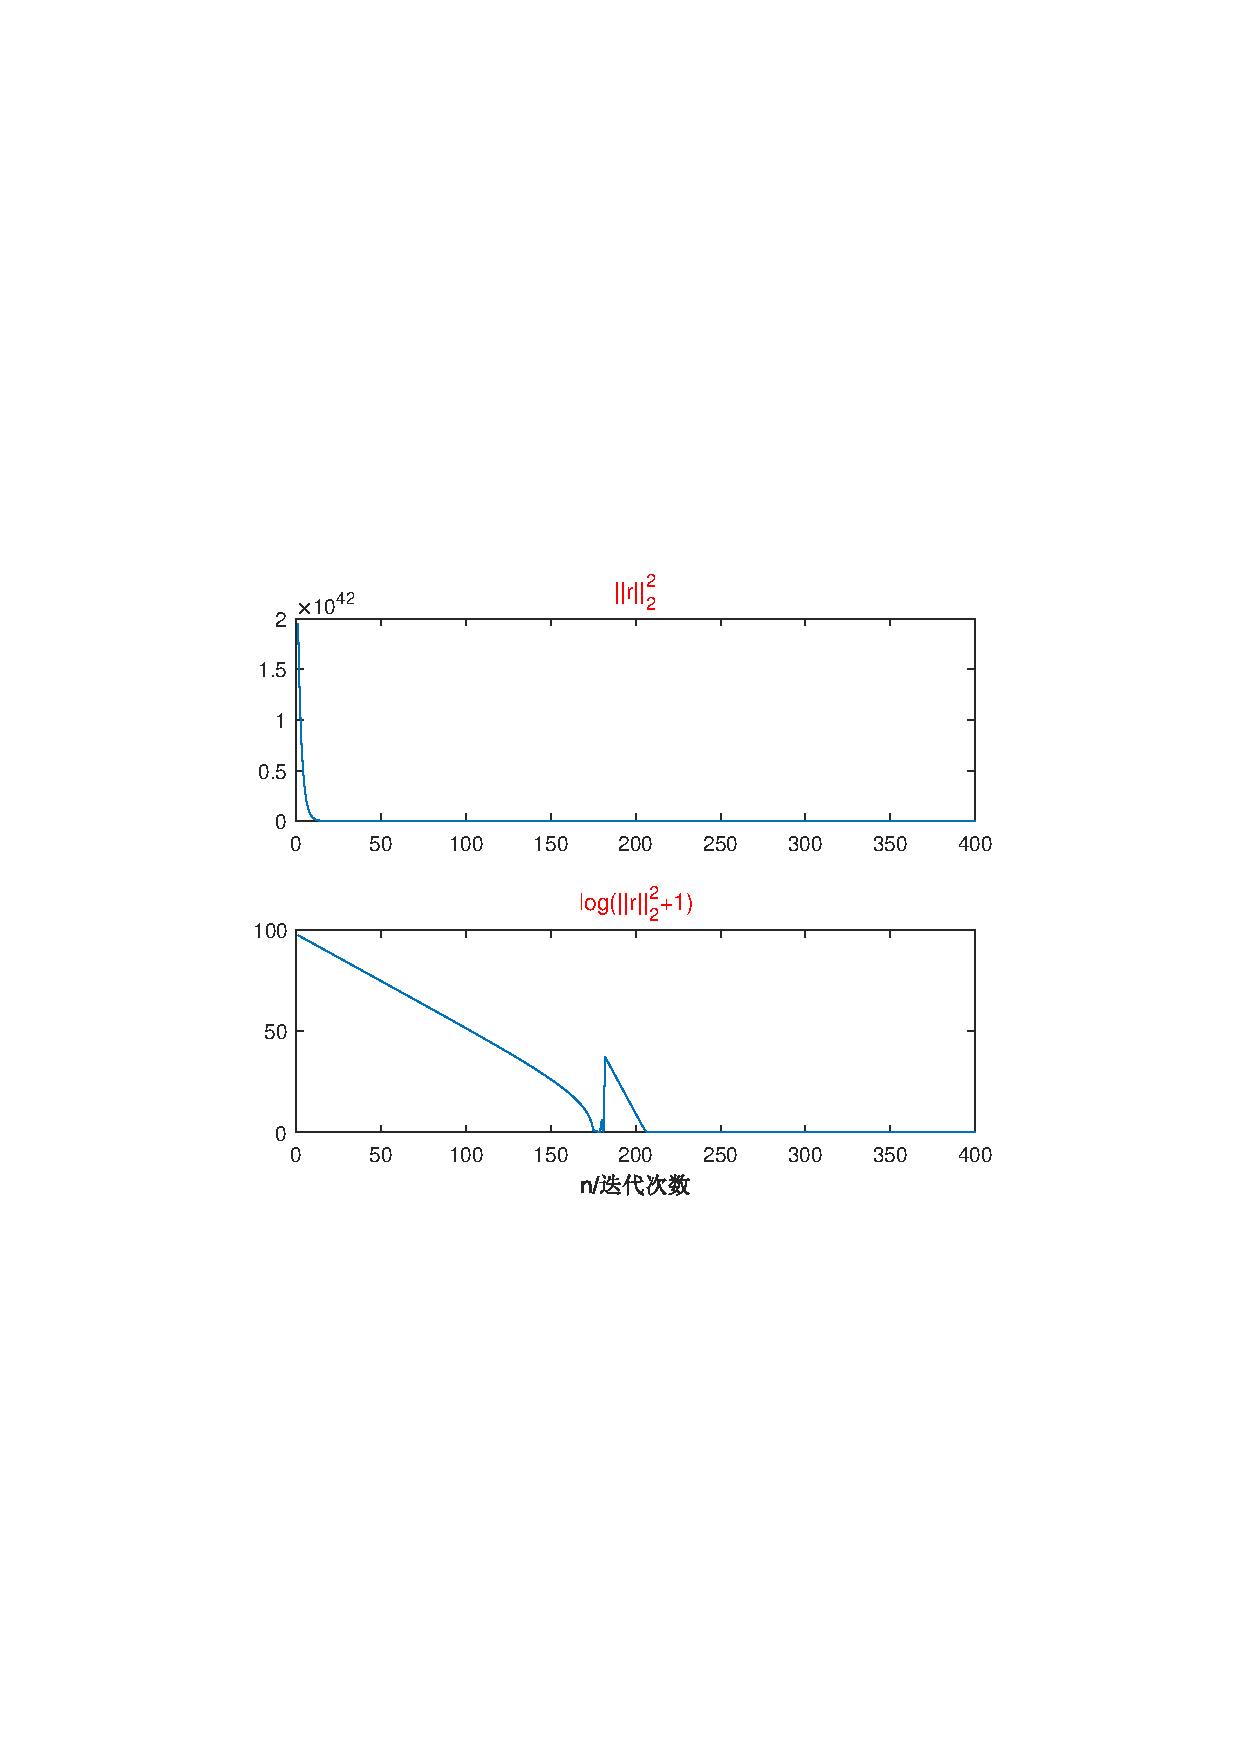
\includegraphics[width=12cm]{1.pdf}
\end{figure}



又采用MATLAB中优化工具箱中的lsqnonlin函数进行拟合,得到的结果比我的程序算出来的略好,将两者进行比较,比较结果如下:

\begin{figure}[H]
\centering
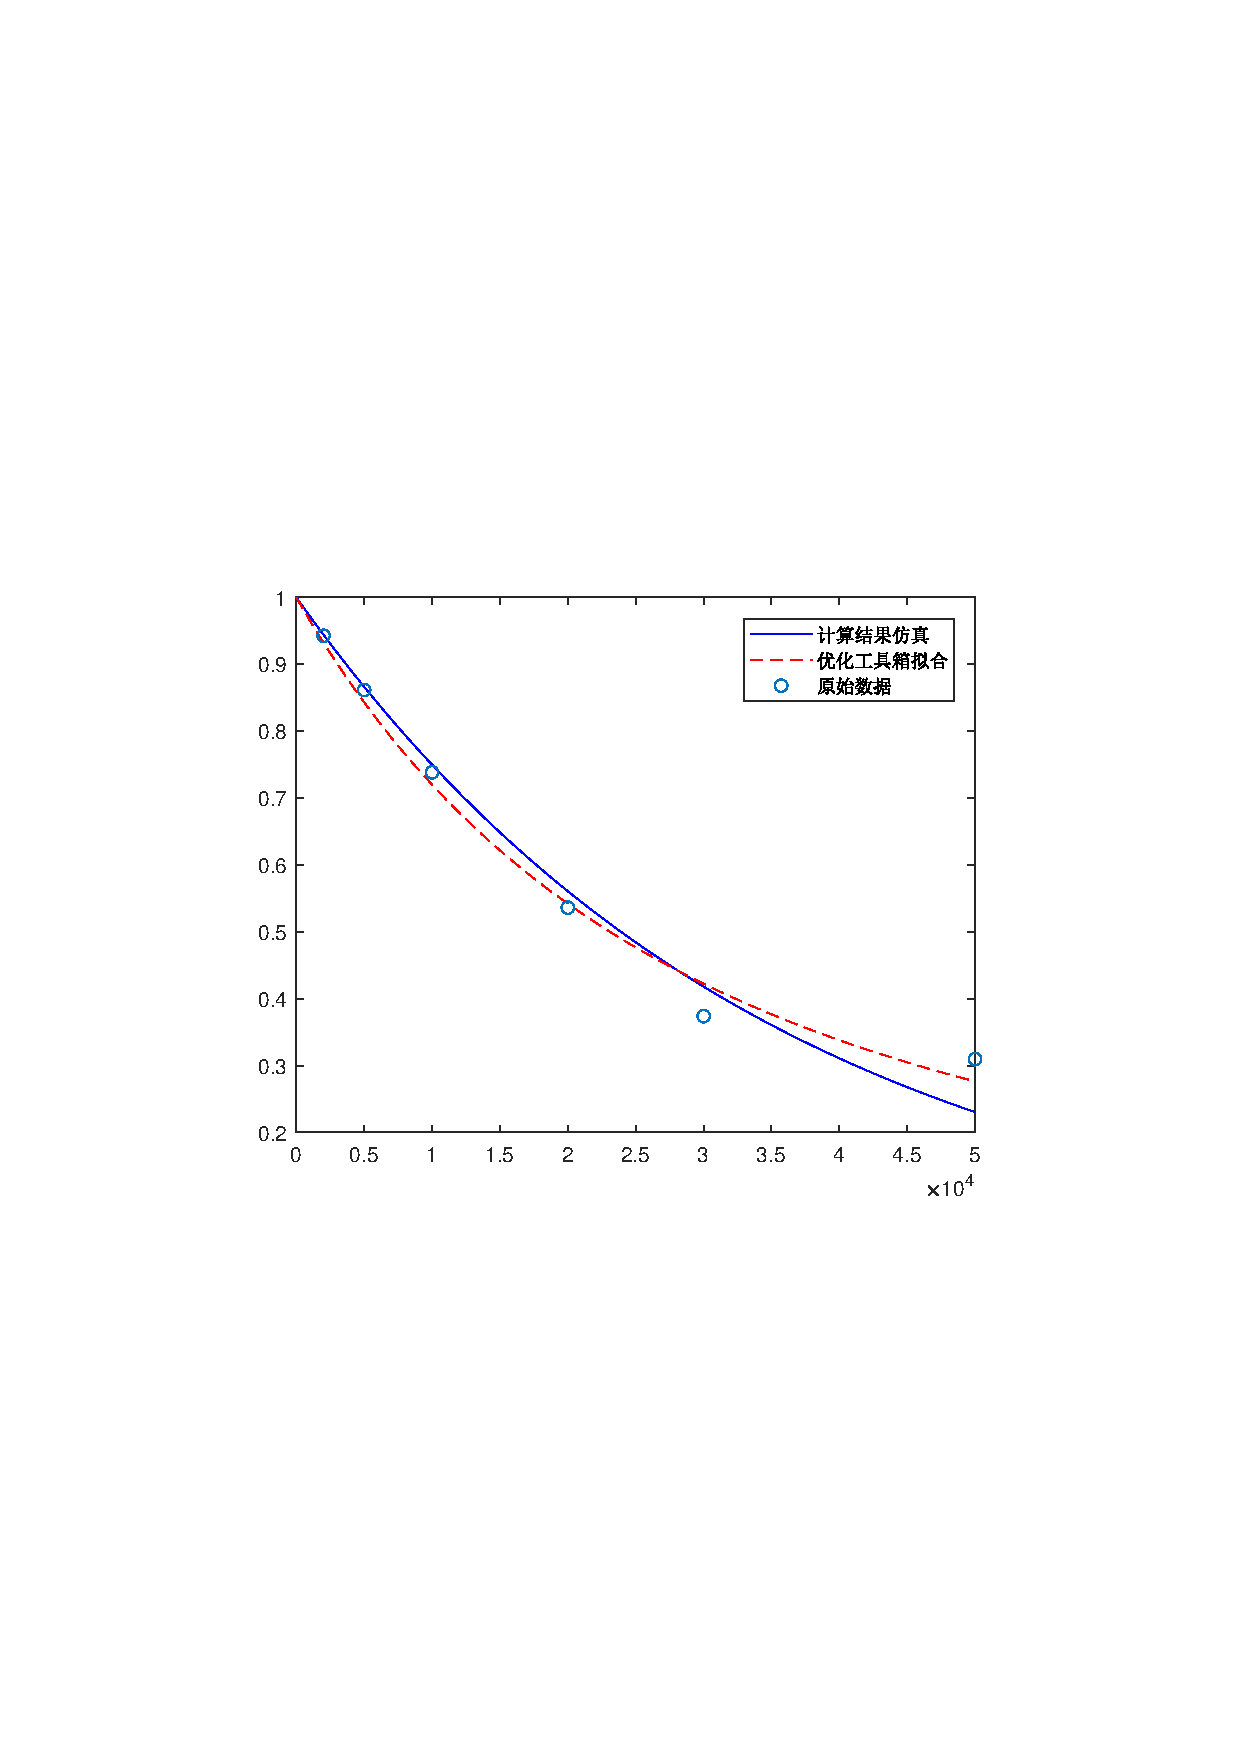
\includegraphics[width=12cm]{2.pdf}
\end{figure}


\begin{table}[H]
\centering
\caption{结果比较}
	\begin{tabular}{ccc}
	\toprule
	{}&程序计算&工具箱拟合\\
	\midrule
	stv&0.125639950119876&0.104420208306470\\
	$x_1$&3.323336983976929e-04&-0.009615612533368\\
	$x_2$&3.516673367231929e+02&-19.446505801429495\\
	\bottomrule
	\end{tabular}
\end{table}



\newpage
\item[6.1]
\[f(x)=10(x_2-x_1^2)^2+(1-x_1)^2\]

\[q(x)=\begin{bmatrix}
-10x_1(x_2-x_1^2)-2(1-x_1)\\
20(x_2-x_1^2)
\end{bmatrix}\]

\[G(x)=\begin{bmatrix}
-40(x_2-x_1^2)+80x_1+2&-40x_1\\
-40x_1&20
\end{bmatrix}\]

\[q(\bm{s})=f^{(k)}+{g^{(k)}}^Ts+\dfrac{1}{2}s^TG^{(k)}s\]

\begin{enumerate}
\item
故对于$\bm{x}^{(k)}=(0,-1)^T$,有:
\[f^{(k)}=11,\quad 
q(x)=\begin{bmatrix}
-2\\
20
\end{bmatrix},\quad 
G(x)=\begin{bmatrix}
42&-0\\
0&20
\end{bmatrix}\]

二次子问题为:

\begin{alignat}{2}
min \quad & q(\bm{s}) \nonumber\\
\mbox{s.t.}\quad
&\|\bm{s}\|_2\leq\Delta \nonumber
\end{alignat}
其中,$q(\bm{s})=21s_1^2+10s_2^2-2s_1-20s_2+11$.

\newpage
\item 
信赖域子问题解族的示意图如下:

\begin{figure}[H]
\centering
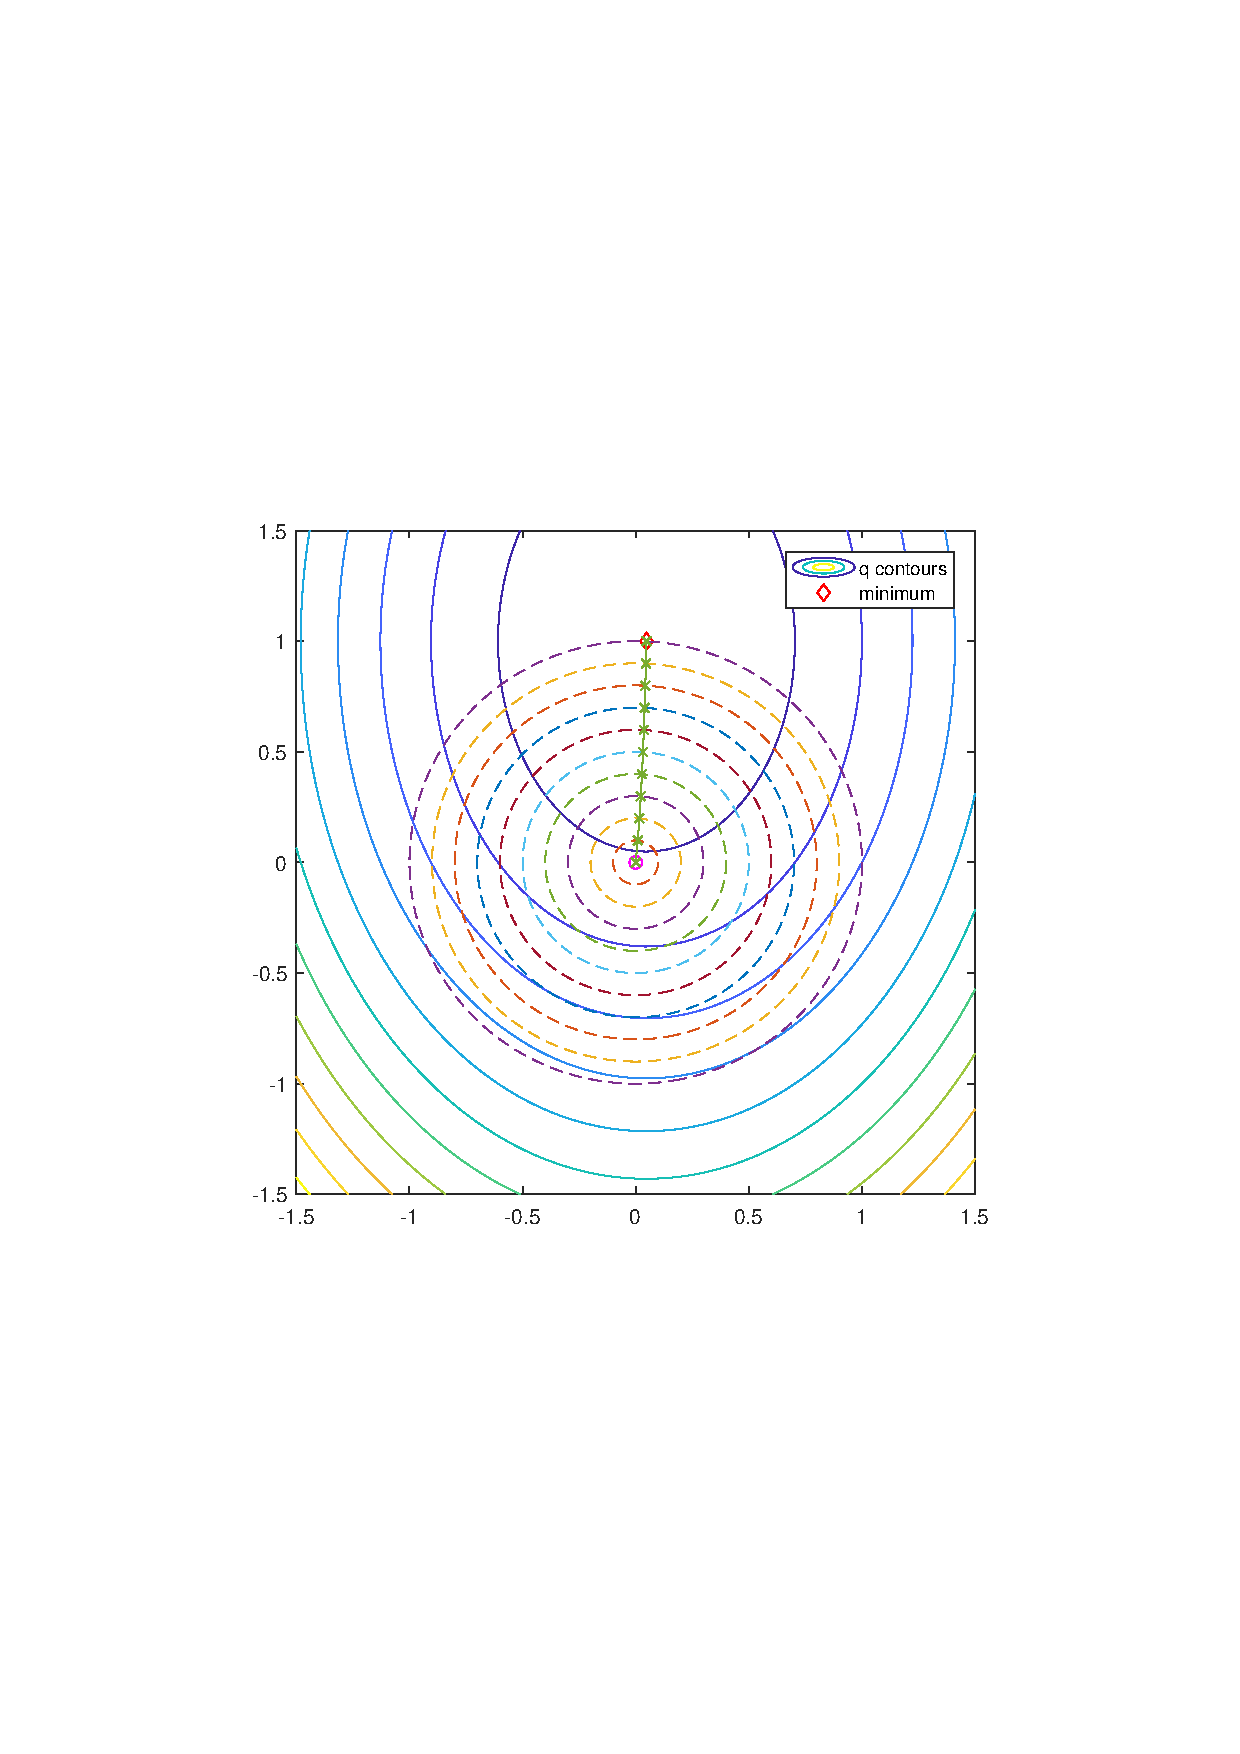
\includegraphics[width=11cm]{3.pdf}
\end{figure}

\item
$\bm{x}^{(k)}$点处的最速下降方向$\bm{p}^{(k)}$为$(2,20)^T$,那么该问题为:

\begin{alignat}{2}
min \quad & q(\alpha \bm{p}^{(k)}) \nonumber\\
\mbox{s.t.}\quad
&\|\alpha \bm{p}^{(k)}\|_2\leq\Delta \nonumber
\end{alignat}
其中,$q(\bm{s})=21s_1^2+10s_2^2-2s_1-20s_2+11$.代入得:

\begin{alignat}{2}
min \quad & 4084\alpha^2-404\alpha+11 \nonumber\\
\mbox{s.t.}\quad
&0\leq \alpha\leq \dfrac{1}{2\sqrt{101}}=0.0498 \nonumber
\end{alignat}

显然,$\alpha=101/2042=0.0495$时,取得最小值,且在信赖域区间内.
故柯西点为$\bm{s_C}=\alpha^{\star} \bm{p}^{(k)}=(\dfrac{101}{1021},\dfrac{1010}{1021})^T$

\item
对于$\bm{x}^{(k)}=(0,0.5)^T$,有:
\[f^{(k)}=3.5,\quad 
q(x)=\begin{bmatrix}
-2\\
10
\end{bmatrix},\quad 
G(x)=\begin{bmatrix}
-18&-0\\
0&20
\end{bmatrix}\]

二次子问题为:

\begin{alignat}{2}
min \quad & q(\bm{s}) \nonumber\\
\mbox{s.t.}\quad
&\|\bm{s}\|_2\leq\Delta \nonumber
\end{alignat}
其中,$q(\bm{s})=-9s_1^2+10s_2^2-2s_1+10s_2+3.5$.

信赖域子问题解族的示意图如下:

\begin{figure}[H]
\centering
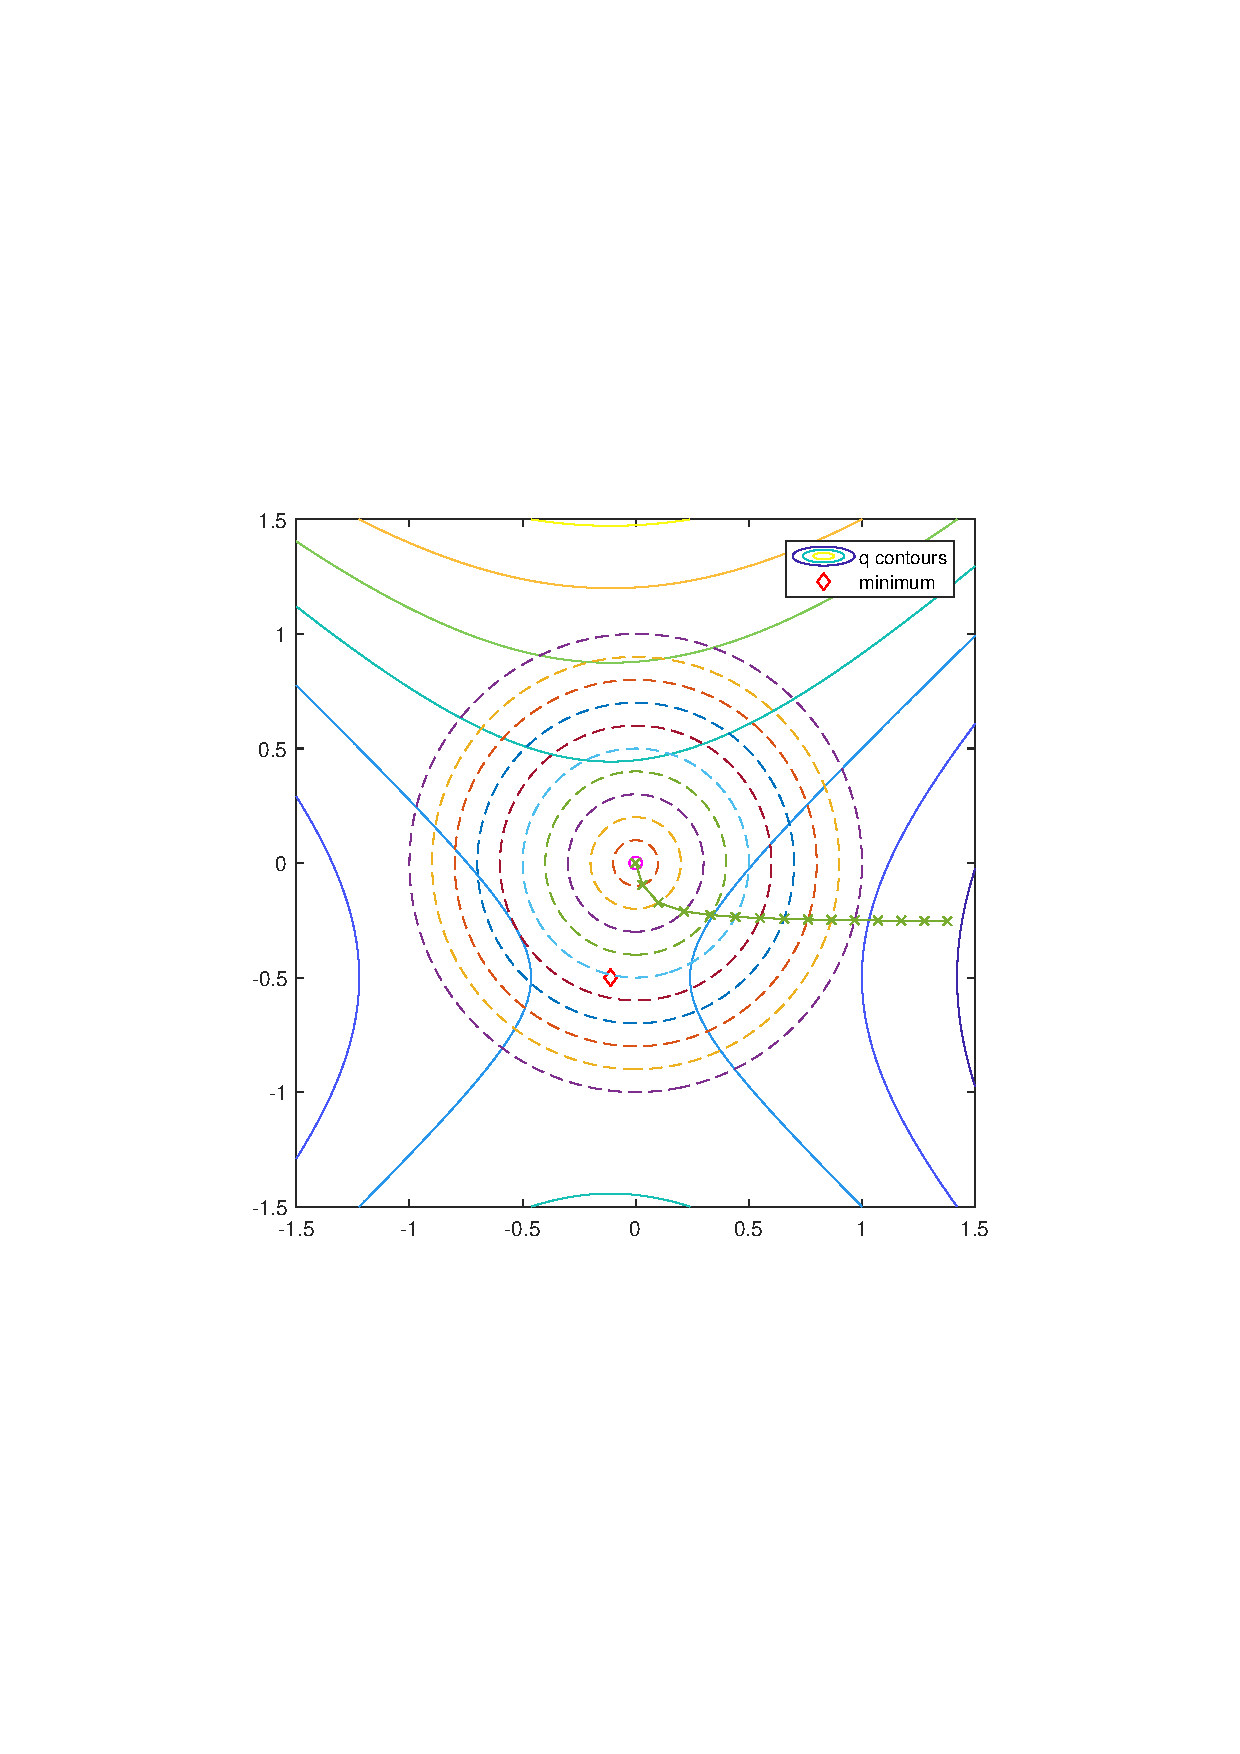
\includegraphics[width=11cm]{4.pdf}
\end{figure}

$\bm{x}^{(k)}$点处的最速下降方向$\bm{p}^{(k)}$为$(2,-10)^T$,那么该问题为:

\begin{alignat}{2}
min \quad & q(\alpha \bm{p}^{(k)}) \nonumber\\
\mbox{s.t.}\quad
&\|\alpha \bm{p}^{(k)}\|_2\leq\Delta \nonumber
\end{alignat}
其中,$q(\bm{s})=-9s_1^2+10s_2^2-2s_1+10s_2+3.5$.代入得:

\begin{alignat}{2}
min \quad & 964\alpha^2-104\alpha+3.5 \nonumber\\
\mbox{s.t.}\quad
&0\leq \alpha\leq \frac{1}{\sqrt{104}}=0.0981 \nonumber
\end{alignat}

显然,$\alpha=13/241=0.0539$时,取得最小值,且在信赖域区间内.
故柯西点为$\bm{s_C}=\alpha^{\star} \bm{p}^{(k)}=(\dfrac{26}{241},\dfrac{-130}{241})^T$
\end{enumerate}

\item[6.2]
\begin{alignat}{2}
min \quad & q(\bm{s})=f+\bm{g}^{T}\bm{s}+\dfrac{\nu}{2}\bm{s}^T\bm{s} \\
\mbox{s.t.}\quad
&\|\bm{s}\|_2\leq\Delta \nonumber
\end{alignat}
\begin{enumerate}
\item 
$\nu=0$时,原问题转化为:
\begin{alignat}{2}
min \quad & q(\bm{s})=f+\bm{g}^{T}\bm{s} \nonumber\\
\mbox{s.t.}\quad
&\|\bm{s}\|_2\leq\Delta \nonumber
\end{alignat}

此时$\bm{s}$的方向为负梯度方向,即
\[\bm{s}^{\star}=-\dfrac{\Delta}{\|\bm{g}\|_2}\bm{g}\]

\item
设$\bm{s}=-\alpha\bm{g}$,代入(1)中得:
\begin{equation}
q(\alpha)=f+(\dfrac{\nu}{2}\alpha^2-\alpha)\bm{g}^T\bm{g}
\end{equation}	
因为$\nu<0$,故$q(\alpha)$在$[0,\dfrac{\Delta}{\|\bm{g}\|_2}]$上单调递减,故$\alpha_{C}=\dfrac{\Delta}{\|\bm{g}\|_2}$,即
\[\bm{s}_{C}=-\dfrac{\Delta}{\|\bm{g}\|_2}\bm{g}\]

\item
对于$\phi(\alpha)=\dfrac{\nu}{2}\alpha^2-\alpha,\quad \alpha\in [0,\dfrac{\Delta}{\|\bm{g}\|_2}]$.

故有:
\[\alpha_{C} = \begin{cases}
\dfrac{\Delta}{\|\bm{g}\|_2},& \dfrac{\Delta}{\|\bm{g}\|_2}\leq \dfrac{1}{\nu}\\
\dfrac{1}{\nu},& \dfrac{\Delta}{\|\bm{g}\|_2}\geq \dfrac{1}{\nu}
\end{cases}\]

\[q(\bm{s}_C)=\begin{cases}
f+\dfrac{\nu}{2}\Delta^2-\|\bm{g}\|_2\Delta,
& \Delta < \dfrac{\|\bm{g}\|_2}{\nu}\\
f-\dfrac{1}{2\nu}\|\bm{g}\|_2^2,& \Delta\geq\dfrac{\|\bm{g}\|_2}{\nu}
\end{cases}\]

而:
\[q(\bm{s}^{\star})=\begin{cases}
f+\dfrac{\nu}{2}\Delta^2-\|\bm{g}\|_2\Delta,
& \Delta < \dfrac{\|\bm{g}\|_2}{\nu}\\
f-\dfrac{1}{2\nu}\|\bm{g}\|_2^2,& \Delta\geq\dfrac{\|\bm{g}\|_2}{\nu}
\end{cases}\]

故:
\[\dfrac{q(\bm{s}_C)}{q(\bm{s}^{\star})}\equiv 1\]

图像如下:
\begin{figure}[H]
\centering
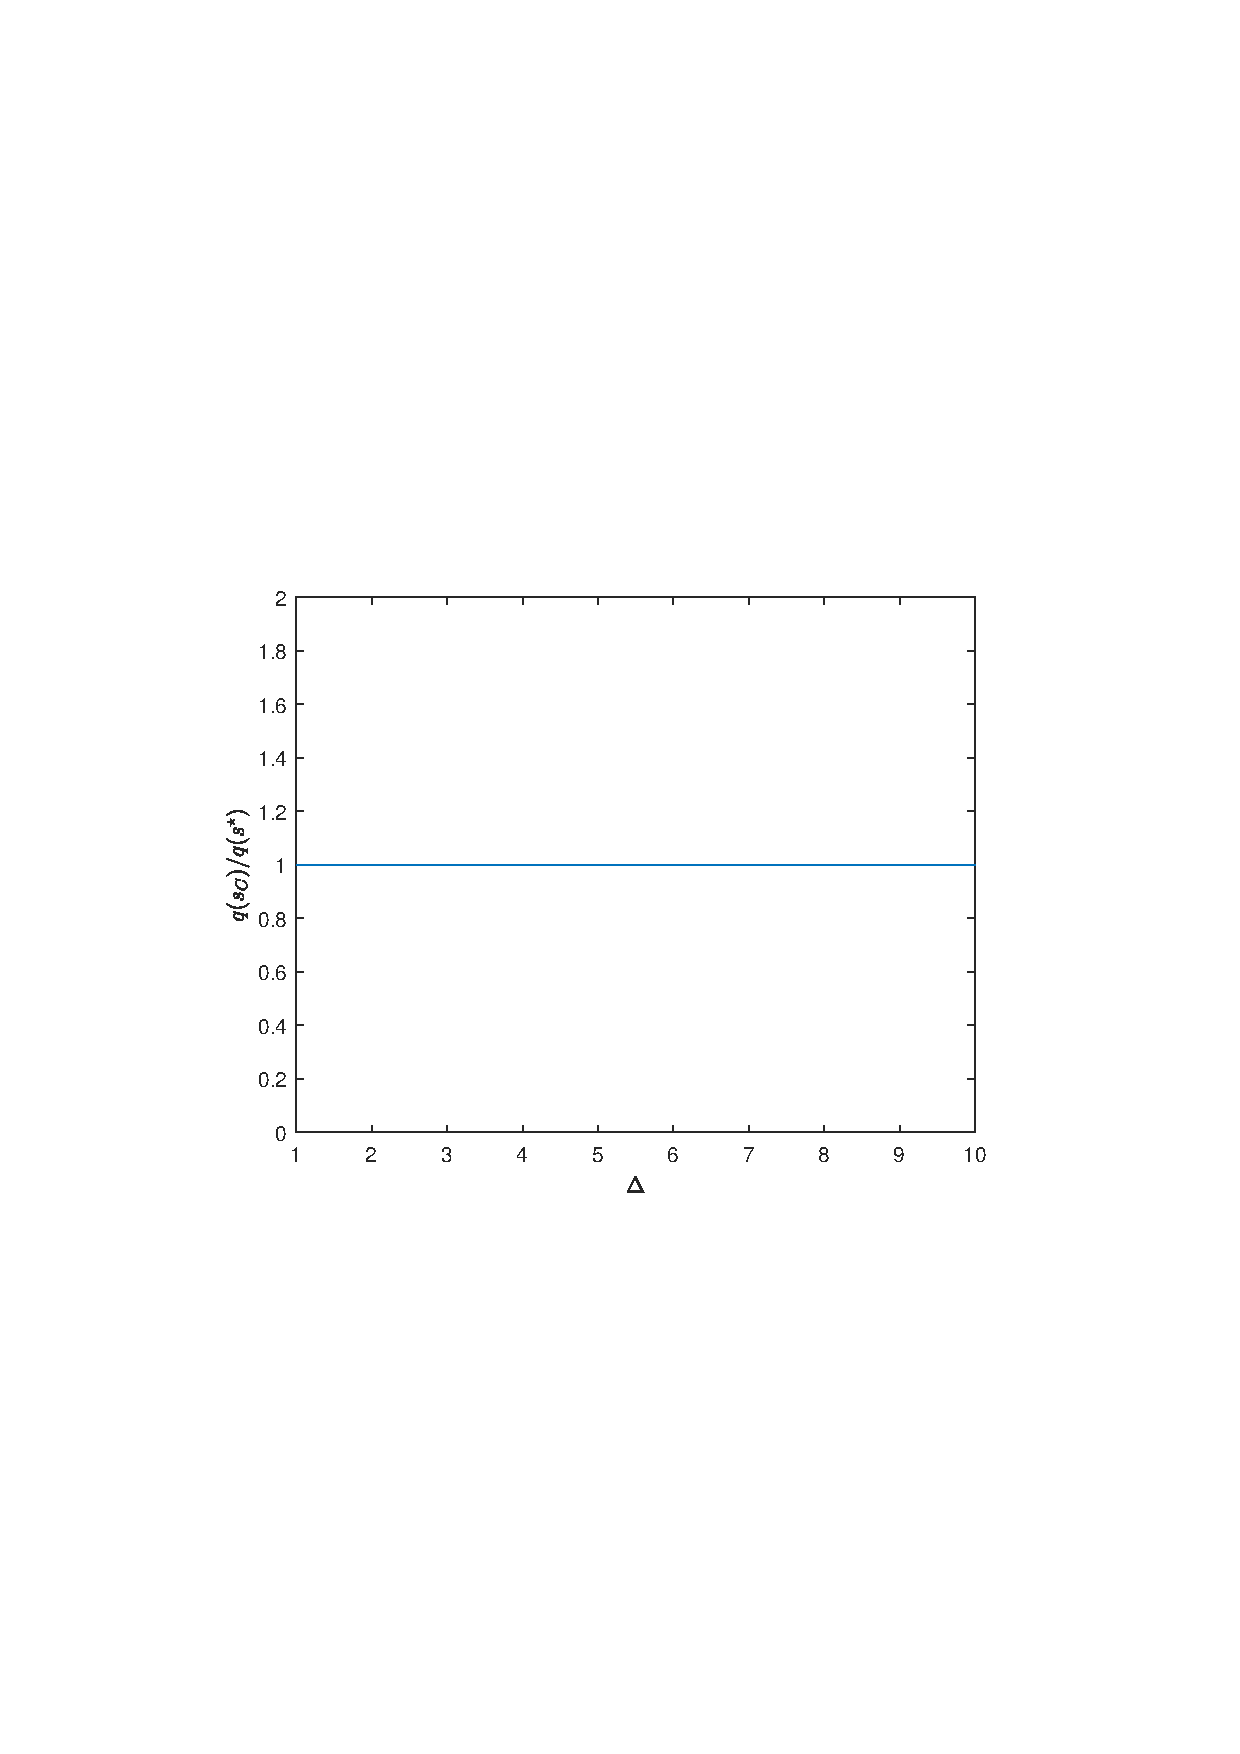
\includegraphics[width=10cm]{5.pdf}
\end{figure}
\end{enumerate}
\end{enumerate}



\newpage
\section*{附录:Matlab代码}

\subsection*{5.27$\quad$GN法}
\begin{lstlisting}[language=Octave]
%	5.27:	GN法
clc;
clear;  %清理工作区变量
N=400;  %设定迭代次数
y=[-1,10];  %设定初始迭代值
d=[0.9427,0.8616,0.7384,0.5362,0.3739,0.3096];
t=[2000,5000,10000,20000,30000,50000];
P=zeros(1,N);%储存残差的下降情况

for step=1:N
    r=rk(y);
    P(step)=norm(r);
    A=d_r(y);
    s=-1*pinv(A'*A)*A'*r;
% 采用Armijo法则计算近似步长ak
%      ak=1;
%       rou=0.01;
%      r1=norm(rk(y+ak*s'));
%     r2=norm(r)+rou*ak*(r'*A*s);
%     while(r1> r2)
%         ak=0.5*ak;
%         r1=norm(rk(y+ak*s'));
%         r2=norm(r)+rou*ak*(r'*A*s);
%     end
    ak=0.05;
    y=y+ak*s';
end
disp('手动计算:')
y;
r=rk(y);
stv=sqrt(norm(r)/6)
x1=1/(y(2)*96.05)
x2=x1/y(1)

figure
subplot(2,1,1);
plot(P)
title('||r||_2^2','Color', 'r')
LP=log(P+1);
subplot(2,1,2);
plot(LP)
xlabel('n/迭代次数')
title('log(||r||_2^2+1)','Color', 'r')

[Y,resnorm] = lsqnonlin(@rk,[-0.5,1]);
disp('工具箱拟合:\n')
Y;
r_opt=rk(Y);
stv_opt=sqrt(norm(r_opt)/6)
x1_opt=1/(Y(2)*96.05)
x2__opt=x1/Y(1)

figure;
X=linspace(0,50000,50);
for i=1:50
y1(i)=phi(X(i),y);
y2(i)=phi(X(i),Y);
end
plot(X,y1,'b')
hold on;
plot(X,y2,'r--')
plot(t,d,'o')
legend('计算结果仿真','优化工具箱拟合','原始数据')



function A=d_r(y)
t=[2000,5000,10000,20000,30000,50000];
A=zeros(6,2);
for i=1:6
    A(i,1:2)=d_ri(t(i),y);
end
end

function dr=d_ri(t,y)
dr=[-1*t*(1-y(1)*t)^(y(2)-2),log(1-y(1)*t)*(1-y(1)*t)^(y(2)-1)];
end

function r=rk(y)
d=[0.9427,0.8616,0.7384,0.5362,0.3739,0.3096];
t=[2000,5000,10000,20000,30000,50000];
r=zeros(6,1);
for i=1:6
    r(i,1)=ri(t(i),y,d(i));
end
end

function r=ri(t,y,di)
r=phi(t,y)-di;
end

function z=phi(t,y)
z=(1-t*y(1))^(y(2)-1);
end
\end{lstlisting}

\subsection*{6.1a}
\begin{lstlisting}[language=Octave]
clc;
clear;
global d;
N=20;
q = @(x) 21*x(1).^2+10*x(2).^2-2*x(1)-20*x(2)+11;
qq = @(x,y) 21*x.^2+10*y.^2-2*x-20*y+11;
fcontour(qq,[-1.5 1.5 -1.5 1.5])
hold on;
plot(1/21,1,'rd')
plot(0,0,'mo')
P=zeros(N+1,2);
x0=[0,0];
lb=[-10,-10];
ub=[10,10];
x2=1+(1/21)^2;
for i=1:N
    d=i/10;
    P(i+1,:) = fmincon(q,x0,[],[],[],[],lb,ub,@circlecon);
    if d^2<=x2
        fimplicit(@(x,y) x.^2+y.^2-d^2,'--')
    end
end
plot(P(:,1),P(:,2),'-x')
legend('q contours','minimum')

function [c,ceq] = circlecon(x)
global d;
c = x(1)^2+x(2)^2-d^2;
ceq = [];
end
\end{lstlisting}

\subsection*{6.1b}
\begin{lstlisting}[language=Octave]
clc;
clear;
global d;
N=14;
size=1.5;
q = @(x) -9*x(1).^2+10*x(2).^2-2*x(1)+10*x(2)+3.5;
qq = @(x,y) -9*x.^2+10*y.^2-2*x+10*y+3.5;
fcontour(qq,[-size size -size size])
hold on;
plot(-1/9,-1/2,'rd')
plot(0,0,'mo')
P=zeros(N+1,2);
x0=[0,0];
lb=[-10,-10];
ub=[10,10];
x2=1/81+1/4;
for i=1:N
    d=i/10;
    P(i+1,:) = fmincon(q,x0,[],[],[],[],lb,ub,@circlecon);
    if d^2<=1
        fimplicit(@(x,y) x.^2+y.^2-d^2,'--')
    end
end
plot(P(:,1),P(:,2),'-x')
legend('q contours','minimum')

function [c,ceq] = circlecon(x)
global d;
c = x(1)^2+x(2)^2-d^2;
ceq = [];
end
\end{lstlisting}
\end{document}